\documentclass[11pt]{article}

\usepackage[margin=1in]{geometry}
\usepackage{amsmath, amssymb, amsthm}
\usepackage{booktabs}
\usepackage{graphicx}
\usepackage{caption}
\usepackage{float}
\usepackage[dvipsnames]{xcolor}
\usepackage{hyperref}
\usepackage{natbib}
\usepackage{bm}
\usepackage{enumitem}

\hypersetup{colorlinks=true, linkcolor=MidnightBlue, urlcolor=MidnightBlue,
            citecolor=MidnightBlue}

\newcommand{\E}{\mathbb{E}}
\newcommand{\Cov}{\operatorname{Cov}}
\newcommand{\Var}{\operatorname{Var}}
\newcommand{\Lproj}{\mathbb{L}}
\newcommand{\perpsym}{^{\perp}}

\title{Replication and Reanalysis of \\
  \emph{The Oregon Health Insurance Experiment}
  \citep{Finkelstein2012}}
\author{Wendy Yin \\ MGTECON 614, Spring 2026}
\date{April 2026}

\begin{document}
\maketitle

% ========================================================================
\section{The paper}

\citet{Finkelstein2012} study the one-year effects of expanding access
to Medicaid using a unique natural experiment. In 2008, Oregon reopened
its \emph{Oregon Health Plan} (OHP) Standard Medicaid program for
low-income, able-bodied adults. Because demand for the program exceeded
its capacity, the state allocated the right to apply through a lottery.
Of the $89{,}824$ individuals on the lottery list, roughly $35{,}000$
were drawn; selection raised the probability of having Medicaid coverage
during the study period by approximately $25$ percentage points.
Lottery assignment is therefore a randomized encouragement to enroll in Medicaid,
which the authors use to estimate (i) intent-to-treat (ITT) effects of
\emph{winning} the lottery and (ii) local average treatment effects
(LATE) of \emph{Medicaid coverage}, instrumenting coverage with the
lottery indicator.

\paragraph{Data.} The analysis combines four sources:
(i) hospital-discharge administrative records for all of Oregon;
(ii) credit-report data from TransUnion;
(iii) Oregon mortality records; and
(iv) a mail survey fielded approximately 14 months after notification,
with $N\!\approx\!23{,}700$ responders and a 50\% effective response
rate. The survey regressions below use the published survey weights.

\paragraph{Empirical specification.} The ITT regression is
\begin{equation}\label{eq:itt}
y_{ihj} \;=\; \beta_{0} + \beta_{1}\,\text{LOTTERY}_{h}
              + X_{ih}'\beta_{2} + V_{ih}'\beta_{3} + \varepsilon_{ihj},
\end{equation}
where $X_{ih}$ contains household-size indicators (and, for survey data,
survey-wave dummies and wave $\times$ household-size interactions; for
administrative data, lottery-draw fixed effects), standard errors are
clustered at the household level, and survey regressions are weighted
to account for the two-arm intensive-follow-up design. The LATE is
estimated by 2SLS with $\text{LOTTERY}_{h}$ instrumenting for an
indicator of insurance coverage:
\begin{equation}\label{eq:iv}
y_{ihj} \;=\; \pi_{0} + \pi_{1}\,\text{INSURANCE}_{ih}
              + X_{ih}'\pi_{2} + V_{ih}'\pi_{3} + \nu_{ihj}.
\end{equation}

\paragraph{Findings.}
\begin{itemize}[leftmargin=*,itemsep=2pt]
  \item \textbf{First stage.} Lottery selection raises ``ever enrolled
  in Medicaid'' by about $25$~pp overall and $29$~pp in the survey
  sub-sample.
  \item \textbf{Utilization (administrative).} Medicaid raises
  non-childbirth hospital admissions by $2.1$~pp ($\approx\!30\%$),
  with no detectable change in admissions originating in the emergency
  department.
  \item \textbf{Survey utilization.} Large increases in
  prescription-drug use, outpatient visits, and preventive-care
  compliance, but no detectable change in ER or inpatient utilization
  over six months.
  \item \textbf{Financial strain.} Lower out-of-pocket medical
  spending, fewer unpaid bills, and a $25\%$ decline in the probability
  of unpaid medical collections, with no change in non-medical
  collections.
  \item \textbf{Health and well-being.} Statistically significant
  improvements across all seven self-reported physical and mental
  health measures, a $32\%$ increase in reporting being ``very or
  pretty happy,'' and no detectable change in mortality over $16$
  months.
\end{itemize}

% ========================================================================
\section{Replication}

\subsection{What can and cannot be replicated}

The OHIE public-use files release individual-level lottery,
state-program, and survey data, but exclude the identifiable
administrative hospital records, credit-report data, and ZIP-level
residence variables used in parts of the original analysis.
Table~\ref{tab:replicability} summarises the implication for each
published table.

\begin{table}[H]\centering\footnotesize
\caption{Replicability of each table in \citet{Finkelstein2012} from
the public release.}
\label{tab:replicability}
\begin{tabular}{llp{0.48\textwidth}}
\toprule
Table & Content & Replicable from public data? \\
\midrule
I    & Control demographics                  & Partial: ZIP income row not in the public files \\
II   & Balance tests                         & Partial: response outcomes only; full F-tests need nonpublic fields \\
III  & First-stage estimates                 & Cols.\ 1--2, 5--6 only (credit cols.\ 3--4 missing) \\
IV   & Hospital utilization (administrative) & \textbf{No} (admin discharge data not public) \\
V    & Health-care utilization (survey)      & \textbf{Yes} \\
VI   & Preventive-care compliance            & \textbf{Yes} \\
VII  & Financial strain (credit reports)     & \textbf{No} (credit data not public) \\
VIII & Financial strain (survey)             & \textbf{Yes} \\
IX   & Health: mortality + survey            & \textbf{Yes} \\
X    & Mechanisms (access, quality, happy)   & \textbf{Yes} \\
XI   & Effects at different times            & \textbf{Yes} \\
\bottomrule
\end{tabular}
\end{table}

\subsection{Implementation}

All estimates below are computed in Python from the public-use
\texttt{.dta} files, without using the authors' Stata \texttt{.do}
files. The specifications use OLS or 2SLS with household-clustered
standard errors. Full-sample first-stage rows control for lottery draw
and household size. Survey regressions use survey-wave $\times$
household-size fixed effects and the published survey-response weights.
The full lottery sample contains $N=74{,}922$ individuals ($29{,}834$
lottery winners); the 12-month survey sub-sample contains $N=23{,}741$
responders. The
first-stage regression of ``ever enrolled in Medicaid'' on the lottery
indicator (survey sub-sample) yields $\hat{\delta}_{1}=0.290$ (SE
$0.007$), with first-stage $F$-statistic well above $500$ and a
control-group enrolment rate of $0.135$.

\subsection{Replication results}

Tables~\ref{tab:rep-I}--\ref{tab:rep-XI} report all replication
results that can be constructed from the public-use files. Table~I is
descriptive and is reproduced up to rows that require nonpublic
ZIP-income information. Table~III is reported for the full-sample and
survey-respondent columns; the credit-report column is not available in
the public release. Tables~V, VI, VIII, IX, X, and XI are survey or
state-program results and are reproduced directly from the public
files. Across these rows, the point estimates match the published
rounded values to the reported precision, except for the TANF/SNAP
public-program rows in Table~III, which are reported as public-file
estimates and not used in the reanalysis.

% Written by code/extra_replications.py. Do not edit by hand.
\begin{table}[H]\centering\scriptsize
\caption{Replication of \citet{Finkelstein2012} Table I: control-group descriptive statistics available in the public files.}
\label{tab:rep-I}
\begin{tabular}{lr}
\toprule
Variable & Control mean \\
\midrule
\multicolumn{2}{l}{\textit{Panel A: full sample}} \\
\% Female & 0.557 \\
\% 50-64 & 0.267 \\
\% 20-50 & 0.733 \\
\% English preferred & 0.922 \\
\% MSA & 0.773 \\
ZIP median household income & Not in public files \\
\midrule
\multicolumn{2}{l}{\textit{Panel B: survey responders}} \\
Lottery list: \% Female & 0.591 \\
Lottery list: \% 50-64 & 0.316 \\
Lottery list: \% 20-50 & 0.684 \\
Lottery list: \% English & 0.917 \\
Lottery list: \% MSA & 0.751 \\
Lottery list: ZIP median household income & Not in public files \\
Survey: \% White & 0.820 \\
Survey: \% Black & 0.038 \\
Survey: \% Hispanic/Latino & 0.123 \\
Survey: ever diagnosed diabetes & 0.175 \\
Survey: ever diagnosed asthma & 0.276 \\
Survey: ever diagnosed high blood pressure & 0.399 \\
Survey: ever diagnosed emphysema/chronic bronchitis & 0.129 \\
Survey: ever diagnosed depression/anxiety & 0.557 \\
Survey: education less than high school & 0.177 \\
Survey: education high school/GED & 0.491 \\
Survey: education vocational/2-year & 0.220 \\
Survey: education 4-year college or more & 0.112 \\
Survey: income <50\% FPL & 0.406 \\
Survey: income 50-75\% FPL & 0.138 \\
Survey: income 75-100\% FPL & 0.140 \\
Survey: income 100-150\% FPL & 0.177 \\
Survey: income above 150\% FPL & 0.139 \\
Survey: average household income & Not in public files \\
Survey: \% Any insurance & 0.325 \\
Survey: \% OHP/Medicaid & 0.117 \\
Survey: \% Private & 0.128 \\
Survey: \% Other insurance & 0.102 \\
Survey: \# months of last 6 insured & 1.738 \\
\bottomrule
\end{tabular}
\end{table}
% Written by code/replicate_tables.py. Do not edit by hand.

\paragraph{Table III: first stage and public-program outcomes.}
Table~\ref{tab:rep-III} reports the first-stage rows that can be constructed from the public files. The Medicaid and self-reported insurance rows reproduce the published values. The TANF/SNAP rows are reported as public-file estimates; these rows do not match the published values as closely, so I do not use them in the reanalysis. The credit-report column in the published table is not reproduced because those data are not public.

\begin{table}[H]\centering\scriptsize
\caption{Replication of \citet{Finkelstein2012} Table III: first-stage estimates in the public files. Each cell reports mine (SE) / paper.}
\label{tab:rep-III}
\resizebox{\textwidth}{!}{%
\begin{tabular}{lrrrr}
\toprule
Outcome & Full control & Full FS & Survey control & Survey FS \\
\midrule
Ever on Medicaid & 0.141 / 0.141 & 0.256\textsuperscript{***} (0.004) / 0.256 & 0.135 / 0.135 & 0.290\textsuperscript{***} (0.007) / 0.290 \\
Ever on OHP Standard & 0.027 / 0.027 & 0.264\textsuperscript{***} (0.003) / 0.264 & 0.026 / 0.026 & 0.302\textsuperscript{***} (0.005) / 0.302 \\
\# months on Medicaid & 1.408 / 1.408 & 3.355\textsuperscript{***} (0.045) / 3.355 & 1.509 / 1.509 & 3.943\textsuperscript{***} (0.090) / 3.943 \\
On Medicaid, end of study period & 0.106 / 0.106 & 0.148\textsuperscript{***} (0.003) / 0.148 & 0.105 / 0.105 & 0.189\textsuperscript{***} (0.006) / 0.189 \\
Currently have any insurance (self-report) &  &  & 0.325 / 0.325 & 0.179\textsuperscript{***} (0.008) / 0.179 \\
Currently have private insurance (self-report) &  &  & 0.128 / 0.128 & -0.008 (0.005) / -0.008 \\
Currently on Medicaid (self-report) &  &  & 0.117 / 0.117 & 0.197\textsuperscript{***} (0.006) / 0.197 \\
Currently on Medicaid &  &  & 0.105 / 0.105 & 0.191\textsuperscript{***} (0.006) / 0.191 \\
Ever on TANF & 0.031 / 0.031 & 0.002 (0.001) / 0.001 & 0.023 / 0.023 & 0.002 (0.003) / 0.002 \\
TANF benefits (\$) & 124.049 / 124.000 & 2.338 (6.527) / -1.659 & 99.686 / 100.000 & 4.281 (11.961) / -4.991 \\
Ever on food stamps & 0.606 / 0.606 & 0.028\textsuperscript{***} (0.004) / 0.017 & 0.622 / 0.622 & 0.027\textsuperscript{***} (0.008) / 0.023 \\
Food stamp benefits (\$) & 1776.281 / 1776.000 & 95.363\textsuperscript{***} (20.686) / 61.300 & 2202.239 / 2202.000 & 96.995\textsuperscript{**} (46.482) / 122.400 \\
\bottomrule
\end{tabular}
}
\end{table}

\begin{table}[H]\centering\scriptsize
\caption{Replication of \citet{Finkelstein2012} Table V: health-care utilization, survey data.}
\label{tab:rep-V}
\resizebox{\textwidth}{!}{%
\begin{tabular}{llrrrrrr}
\toprule
Panel & Outcome & Control & ITT & ITT & LATE & LATE & \\
 & & mean & (mine) & (paper) & (mine, SE) & (paper) & $N$ \\
\midrule
 & Prescription drugs currently & 0.637 & 0.025 & 0.025 & 0.088\textsuperscript{***} (0.029) & 0.088 & 18{,}308 \\
 & Outpatient visits last 6m & 0.574 & 0.062 & 0.062 & 0.212\textsuperscript{***} (0.025) & 0.212 & 23{,}492 \\
 & ER visits last 6m & 0.261 & 0.006 & 0.006 & 0.022 (0.023) & 0.022 & 23{,}514 \\
 & Inpatient hosp. admissions last 6m & 0.072 & 0.002 & 0.002 & 0.008 (0.014) & 0.008 & 23{,}573 \\
 & \# Prescription drugs & 2.318 & 0.100 & 0.100 & 0.347\textsuperscript{**} (0.176) & 0.347 & 18{,}297 \\
 & \# Outpatient visits & 1.914 & 0.314 & 0.314 & 1.083\textsuperscript{***} (0.182) & 1.083 & 23{,}441 \\
 & \# ER visits & 0.470 & 0.007 & 0.007 & 0.026 (0.056) & 0.026 & 23{,}481 \\
 & \# Inpatient admissions & 0.097 & 0.006 & 0.006 & 0.021 (0.021) & 0.021 & 23{,}539 \\
\bottomrule
\end{tabular}
}
\end{table}

\begin{table}[H]\centering\scriptsize
\caption{Replication of \citet{Finkelstein2012} Table VI: compliance with recommended preventive care.}
\label{tab:rep-VI}
\resizebox{\textwidth}{!}{%
\begin{tabular}{llrrrrrr}
\toprule
Panel & Outcome & Control & ITT & ITT & LATE & LATE & \\
 & & mean & (mine) & (paper) & (mine, SE) & (paper) & $N$ \\
\midrule
 & Blood cholesterol checked (ever) & 0.625 & 0.033 & 0.033 & 0.114\textsuperscript{***} (0.026) & 0.114 & 23{,}390 \\
 & Blood tested for high blood sugar/diab. & 0.604 & 0.026 & 0.026 & 0.090\textsuperscript{***} (0.026) & 0.090 & 23{,}374 \\
 & Mammogram within last 12m (women>=40) & 0.298 & 0.055 & 0.055 & 0.184\textsuperscript{***} (0.040) & 0.187 & 7{,}927 \\
 & Pap test within last 12m (women) & 0.406 & 0.051 & 0.051 & 0.183\textsuperscript{***} (0.034) & 0.183 & 13{,}924 \\
\bottomrule
\end{tabular}
}
\end{table}

\begin{table}[H]\centering\scriptsize
\caption{Replication of \citet{Finkelstein2012} Table VIII: financial strain, survey data.}
\label{tab:rep-VIII}
\resizebox{\textwidth}{!}{%
\begin{tabular}{llrrrrrr}
\toprule
Panel & Outcome & Control & ITT & ITT & LATE & LATE & \\
 & & mean & (mine) & (paper) & (mine, SE) & (paper) & $N$ \\
\midrule
 & Any OOP medical expenses, last 6m & 0.555 & -0.058 & -0.058 & -0.200\textsuperscript{***} (0.026) & -0.200 & 23{,}426 \\
 & Owe money for medical expenses currently & 0.597 & -0.052 & -0.052 & -0.180\textsuperscript{***} (0.026) & -0.180 & 23{,}451 \\
 & Borrowed/skipped bills for medical debt, last 6m & 0.364 & -0.045 & -0.045 & -0.154\textsuperscript{***} (0.025) & -0.154 & 23{,}410 \\
 & Refused treatment because of medical debt, last 6m & 0.081 & -0.011 & -0.011 & -0.036\textsuperscript{**} (0.014) & -0.036 & 22{,}571 \\
\bottomrule
\end{tabular}
}
\end{table}

\begin{table}[H]\centering\scriptsize
\caption{Replication of \citet{Finkelstein2012} Table IX: mortality and self-reported health.}
\label{tab:rep-IX}
\resizebox{\textwidth}{!}{%
\begin{tabular}{llrrrrrr}
\toprule
Panel & Outcome & Control & ITT & ITT & LATE & LATE & \\
 & & mean & (mine) & (paper) & (mine, SE) & (paper) & $N$ \\
\midrule
A & Alive through September 2009 & 0.992 & 0.000 & 0.000 & 0.001 (0.003) & 0.001 & 74{,}922 \\
B & Self-reported health good/VG/excellent & 0.548 & 0.039 & 0.039 & 0.133\textsuperscript{***} (0.026) & 0.133 & 23{,}361 \\
B & Self-reported health not poor & 0.860 & 0.029 & 0.029 & 0.099\textsuperscript{***} (0.018) & 0.099 & 23{,}361 \\
B & Health same/better last 6m & 0.714 & 0.033 & 0.033 & 0.113\textsuperscript{***} (0.023) & 0.113 & 23{,}407 \\
B & \# days physical health good (past 30) & 21.862 & 0.381 & 0.381 & 1.317\textsuperscript{**} (0.563) & 1.317 & 21{,}881 \\
B & \# days not impaired (past 30) & 20.329 & 0.459 & 0.459 & 1.585\textsuperscript{***} (0.606) & 1.585 & 21{,}384 \\
B & \# days mental health good (past 30) & 18.738 & 0.603 & 0.603 & 2.082\textsuperscript{***} (0.640) & 2.082 & 21{,}601 \\
B & Did not screen positive for depression & 0.671 & 0.023 & 0.023 & 0.078\textsuperscript{***} (0.025) & 0.078 & 23{,}147 \\
\bottomrule
\end{tabular}
}
\end{table}

\begin{table}[H]\centering\scriptsize
\caption{Replication of \citet{Finkelstein2012} Table X: access, quality, and happiness.}
\label{tab:rep-X}
\resizebox{\textwidth}{!}{%
\begin{tabular}{llrrrrrr}
\toprule
Panel & Outcome & Control & ITT & ITT & LATE & LATE & \\
 & & mean & (mine) & (paper) & (mine, SE) & (paper) & $N$ \\
\midrule
 & Have usual place of clinic-based care & 0.499 & 0.099 & 0.099 & 0.339\textsuperscript{***} (0.027) & 0.339 & 21{,}541 \\
 & Have personal doctor & 0.490 & 0.081 & 0.081 & 0.280\textsuperscript{***} (0.026) & 0.280 & 23{,}501 \\
 & Got all needed medical care, last 6m & 0.684 & 0.069 & 0.069 & 0.239\textsuperscript{***} (0.022) & 0.239 & 22{,}904 \\
 & Got all needed drugs, last 6m & 0.765 & 0.056 & 0.056 & 0.195\textsuperscript{***} (0.019) & 0.195 & 22{,}825 \\
 & Didn't use ER for nonemergency, last 6m & 0.916 & -0.001 & -0.001 & -0.004 (0.015) & -0.004 & 23{,}530 \\
 & Quality of care good/VG/excellent (conditional) & 0.708 & 0.043 & 0.043 & 0.142\textsuperscript{***} (0.027) & 0.142 & 16{,}316 \\
 & Very happy or pretty happy & 0.594 & 0.056 & 0.056 & 0.191\textsuperscript{***} (0.026) & 0.191 & 23{,}416 \\
\bottomrule
\end{tabular}
}
\end{table}

\paragraph{Table XI: treatment effects at different survey waves.}
Table~\ref{tab:rep-XI} reports standardized ITT effects at the initial, six-month, and main survey waves. Each cell reports mine (SE) / paper.

\begin{table}[H]\centering\scriptsize
\caption{Replication of \citet{Finkelstein2012} Table XI: estimated effects of lottery at different times.}
\label{tab:rep-XI}
\resizebox{\textwidth}{!}{%
\begin{tabular}{lrrr}
\toprule
Domain & Initial survey & Six-month survey & Main survey \\
\midrule
Utilization (extensive margin) & 0.004 (0.009) / 0.004 & 0.047\textsuperscript{*} (0.021) / 0.047 & 0.050\textsuperscript{***} (0.012) / 0.050 \\
Utilization (total) & -0.000 (0.009) / -0.000 & 0.027 (0.021) / 0.027 & 0.040\textsuperscript{***} (0.012) / 0.040 \\
Financial strain & -0.035\textsuperscript{***} (0.010) / -0.035 & -0.099\textsuperscript{***} (0.021) / -0.099 & -0.089\textsuperscript{***} (0.010) / -0.089 \\
Health & 0.042\textsuperscript{***} (0.010) / 0.042 & 0.097\textsuperscript{***} (0.025) / 0.097 & 0.061\textsuperscript{***} (0.012) / 0.061 \\
Access & 0.047\textsuperscript{***} (0.008) / 0.047 & 0.075\textsuperscript{***} (0.020) / 0.075 & 0.119\textsuperscript{***} (0.009) / 0.119 \\
\bottomrule
\end{tabular}
}
\end{table}


\begin{figure}[H]\centering
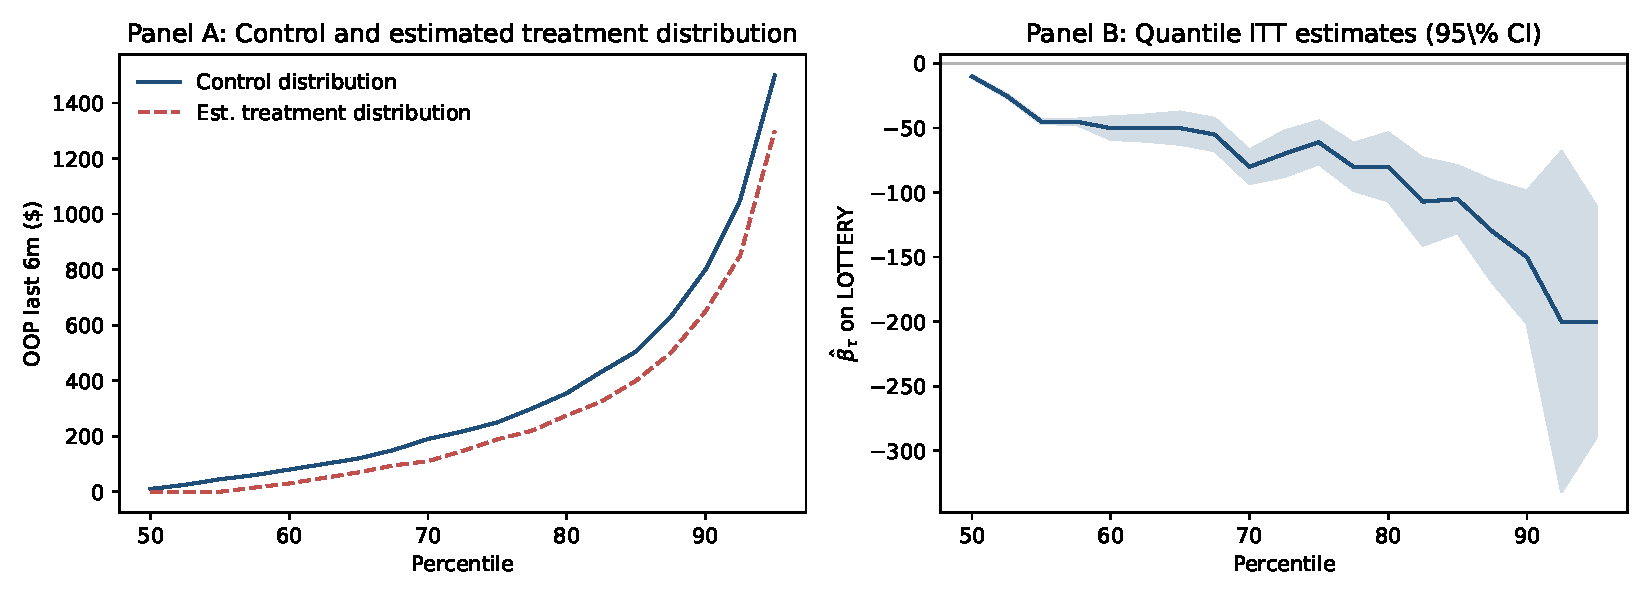
\includegraphics[width=.65\textwidth]{figures/figure1_oop_quantile.pdf}
\caption{Python replication of \citet{Finkelstein2012} Figure~I:
quantile treatment effects on total out-of-pocket medical spending in
the last six months. The figure reproduces the control distribution and
the reduced-form quantile pattern but does not implement the paper's
cluster bootstrap.}
\label{fig:fig1}
\end{figure}

Figure~\ref{fig:fig1} gives a distributional interpretation of the
financial-strain results. The left panel plots the empirical control
distribution of six-month out-of-pocket medical spending and the
estimated treatment distribution obtained by adding the quantile
reduced-form coefficient to the corresponding control quantile. The two
distributions are nearly coincident around the median, where many
respondents report little or no out-of-pocket spending. They separate
in the upper tail: lottery selection shifts the high-spending quantiles
downward. The right panel shows the same result as quantile treatment
effects. The estimates are close to zero at lower quantiles and become
increasingly negative at higher quantiles, which is consistent with
Medicaid reducing exposure to large medical-spending shocks rather than
uniformly lowering spending throughout the distribution.

The replication is sufficiently close that the remaining exercise can
focus on estimator interpretation. The next section asks how the
paper's OLS and 2SLS specifications weight heterogeneous effects, and
what changes when the analysis is restricted to the balanced 0m--12m
panel.

% ========================================================================
\section{Reanalysis}

\subsection{Setup and notation}

Let $Y_{i}$ be one of the four focal survey outcomes used below,
$Z_{i}\in\{0,1\}$ the lottery indicator (\texttt{treatment}),
$D_{i}\in\{0,1\}$ a Medicaid coverage indicator
(\texttt{ohp\_all\_ever}), and $W_{i}$ the saturated stratum
covariates --- by default the set of dummies for survey-wave
($\texttt{draw\_survey\_12m}$) interacted with household size
($\texttt{numhh\_list}$). The household-size controls matter because
Oregon sampled individuals from the lottery list but treated the whole
listed household as eligible to apply when any member was drawn. Survey
regressions use the published survey weights (\texttt{weight\_12m});
standard errors cluster by
\texttt{household\_id}. The four focal outcomes are outpatient visits
in the last six months (\texttt{doc\_num\_mod\_12m}), any out-of-pocket
medical expenditure (\texttt{cost\_any\_oop\_12m}), self-reported
health rated good or better (\texttt{health\_genflip\_bin\_12m}), and
a negative depression screen (\texttt{nodep\_screen\_12m}).

% --------------------------------------------------
\subsection{Heterogeneous-effects decomposition of OLS}

Under the heterogeneous-effect model (HEM)
\[
    Y_{i} \;=\; Z_{i}\,\beta_{i} + g(W_{i}) + \epsilon_{i},
\]
the Frisch--Waugh--Lovell representation of OLS implies
\begin{equation}\label{eq:hem}
    \E[\hat\beta_{\text{OLS}}\mid Z,W] \;=\; \sum_{i} C_{i}\,\beta_{i},
    \qquad
    C_{i} \;=\; \frac{Z_{i}^{\perp}\,Z_{i}}{\sum_{j} (Z_{j}^{\perp})^{2}},
    \qquad \sum_{i} C_{i} = 1,
\end{equation}
where $Z_{i}^{\perp} = Z_{i} - W_{i}'\hat\eta$ is the residual from
regressing $Z$ on $W$. Because $Z$ is binary, $Z_{i}^{\perp} Z_{i} =
Z_{i}(1 - W_{i}'\hat\eta)$, and $C_{i}\ge 0$ as long as
$W_{i}'\hat\eta\le 1$, which holds when $W$ is a saturated set of
assignment-probability cells.
Table~\ref{tab:ols-weights} reports, for each of the focal
specifications, the point estimate, the number of observations
receiving negative ex post weight, the largest weight $\max(n\cdot
C_{i})$, and the effective sample size
$n_{\text{eff}}/n = 1/(n\sum C_{i}^{2})$.

\begin{table}[H]\centering\footnotesize
\caption{Ex post OLS weights under saturated stratum controls.}
\label{tab:ols-weights}
\begin{tabular}{lrrrrr}
\toprule
Regression & $\hat\beta$ & Negative $C_{i}$ & $\max(n\cdot C_{i})$
  & $n_{\text{eff}}/n$ & $n$ \\
\midrule
First stage (Medicaid on lottery)         & $\phantom{-}0.256$ & 0 & 2.87 & 0.38 & 74{,}922 \\
ITT outpatient visits                     & $\phantom{-}0.314$ & 0 & 7.09 & 0.37 & 23{,}441 \\
ITT any OOP medical spending              & $-0.058$           & 0 & 7.09 & 0.37 & 23{,}426 \\
ITT self-reported health good or better   & $\phantom{-}0.039$ & 0 & 7.09 & 0.37 & 23{,}361 \\
ITT negative depression screen            & $\phantom{-}0.023$ & 0 & 7.10 & 0.37 & 23{,}147 \\
\bottomrule
\end{tabular}
\end{table}

\begin{figure}[H]\centering
    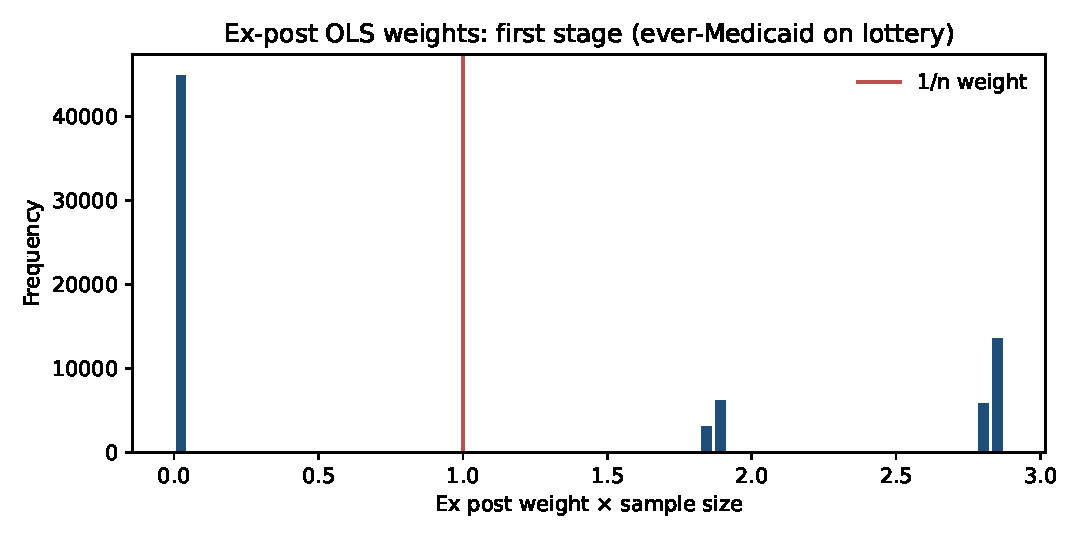
\includegraphics[width=.48\linewidth]{figures/weights_ols_first_stage.pdf}
    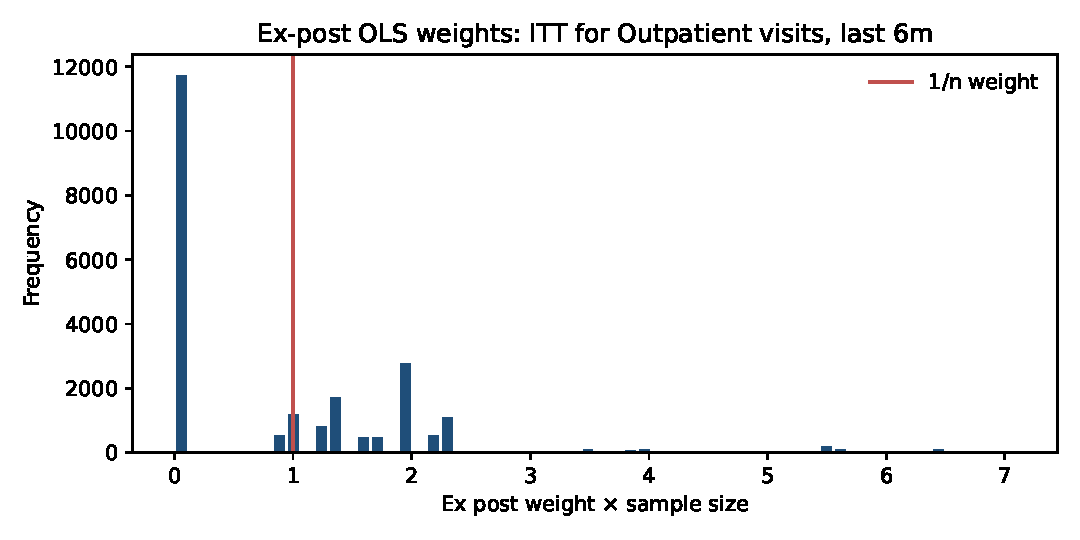
\includegraphics[width=.48\linewidth]{figures/weights_ols_itt_docvisits.pdf}
    \caption{Histograms of ex post OLS weights $n\cdot C_{i}$ for the
    first-stage Medicaid-on-lottery regression (left) and the ITT
    regression of outpatient visits (right). All weights are
    non-negative; the red line marks the $1/n$ baseline.}
    \label{fig:ols-weights}
\end{figure}

Figure~\ref{fig:ols-weights} shows that covariate adjustment does not
create negative OLS weights in the OHIE specifications considered here.
In the first-stage regression, the weights are relatively concentrated:
the maximum observation receives about $2.9/n$, and the effective
sample size is $38\%$ of the nominal full-sample size. The outpatient
ITT regression is more dispersed, with maximum weight about $7.1/n$,
because the survey analysis combines response weights with
survey-wave-by-household-size cells. This dispersion affects precision
and leverage, but not the sign of the causal aggregation: the ITT
coefficient remains a convex weighted average of individual lottery
effects under the saturated control specification.

\paragraph{Ex ante interpretation under the super-population.}
When the assignment model $\E[Z\mid W]$ is linear in $W$ (an assumption
that holds exactly here because $W$ saturates the design), the ex ante
weight on stratum $s$ collapses to
\[
    C(W_{s}) \;=\; \Var(Z\mid W_{s})
              + \E[Z\mid W_{s}]\big(\E[Z\mid W_{s}]
                                       - \Lproj[Z\mid W_{s}]\big)
              \;=\; \Var(Z\mid W_{s})
              \;=\; p_{s}(1-p_{s}),
\]
because saturation implies $\E[Z\mid W]=\Lproj[Z\mid W]$ exactly.
With $17$ randomization strata in the survey sub-sample, the resulting
normalised stratum weights $C(W_{s})/\E[C(W)]$ range over only
$[0.35,\,1.20]$, with a standard deviation of $0.27$, tightly
clustered around one. The stratum weights are therefore close to equal
even though the realized individual weights are dispersed out to
roughly $7/n$.

\paragraph{Why omitted-variable bias vanishes.}
Decomposing the OLS estimand into three terms,
\begin{equation}\label{eq:ovb}
\hat\beta \;=\;
   \underbrace{\sum_{i} C_{i}\beta_{i}}_{\text{weighted causal effect}}
 + \underbrace{\frac{\sum_{i} Z_{i}^{\perp} g(W_{i})}
                    {\sum_{j} (Z_{j}^{\perp})^{2}}}_{\text{omitted-variable bias}}
 + \underbrace{\frac{\sum_{i} Z_{i}^{\perp} \epsilon_{i}}
                    {\sum_{j} (Z_{j}^{\perp})^{2}}}_{\text{residual error}},
\end{equation}
the omitted-variable term is exactly zero when $W$ saturates~$g$,
because $g(W)=W'\xi$ and orthogonality of $Z^{\perp}$ to $W$ then
implies $\sum_{i} Z_{i}^{\perp} W_{i}'\xi = 0$. The residual error has
conditional mean zero by random assignment of the lottery. Hence the
ITT point estimate is a convex combination of individual effects with
no residual confounding.

% --------------------------------------------------
\subsection{2SLS decomposition into complier and always-taker components}

After conditioning on $W$, the 2SLS estimand of the LATE of Medicaid
$D$ on outcome $Y$ admits the
Blandhol--Bonney--Mogstad--Torgovitsky decomposition
\citep{BBMT2022}:
\begin{equation}\label{eq:bbmt}
    \hat\beta_{\text{2SLS}} \;\xrightarrow{p}\;
    \frac{\E\!\left[\, C(W)\,\tau(W) \;+\; C_{a}(W)\,\tau_{a}(W)\,\right]}
         {\E\!\left[\, C(W) + C_{a}(W)\,\right]},
\end{equation}
where $\tau(W) = \E[\Delta Y\mid \Delta D\ne 0,W]$ is the conditional
complier LATE, $\tau_{a}(W)=\E[\Delta Y\mid G=a,W]$ is the
unidentified always-taker effect, and the weights are
\begin{align*}
    C(W)   &= \operatorname{sign}(D(1)-D(0))\cdot
              \E[Z\mid W]\,(1 - \Lproj[Z\mid W])\,\pi(W),\\[2pt]
    C_{a}(W) &= \big(\E[Z\mid W] - \Lproj[Z\mid W]\big)\,\pi_{a}(W).
\end{align*}
The term $C(W)\tau(W)$ is a non-negative re-weighting of the
complier LATE; $C_{a}(W)\tau_{a}(W)$ is contamination from
always-takers. The always-taker term vanishes whenever
$\E[Z\mid W] = \Lproj[Z\mid W]$, which is automatic under a saturated
$W$.

\paragraph{Principal strata in OHIE.}
Under the monotonicity assumption $D(1)\ge D(0)$ almost surely ---
plausible here because a lottery loss does not mechanically deliver
Medicaid through this channel --- the principal-stratum shares in the
survey sub-sample are
\[
    P(D=1\mid Z=1) = 0.426,\qquad
    P(D=1\mid Z=0) = 0.135,\qquad
    \text{first stage} = 0.291,
\]
implying always-takers $\approx 13.5\%$, compliers $\approx 29.1\%$,
and never-takers $\approx 57.4\%$. Thus always-takers are present in
the data; the decomposition checks whether 2SLS gives them nonzero
contamination weight.

\paragraph{Covariate-adjusted 2SLS is not the unconditional LATE.}
The paper's IV estimate is not the raw Wald ratio
$\{\E[Y\mid Z=1]-\E[Y\mid Z=0]\}/\{\E[D\mid Z=1]-\E[D\mid Z=0]\}$.
The authors adjust at least for household size, and for survey outcomes
they adjust for survey-wave $\times$ household-size cells and use survey
weights. This adjustment is necessary for unbiased ITT/first-stage
comparisons because Oregon sampled individuals from the lottery list but
made the selected individual's whole listed household eligible to apply.
Thus the lottery probability varies strongly with household size.

Under monotonicity and saturated covariates, this adjustment removes
always-taker contamination but changes the aggregation of complier
effects:
\[
    \text{unconditional LATE}
      = \frac{\E[\pi(W)\tau(W)]}{\E[\pi(W)]},
    \qquad
    \text{covariate-adjusted 2SLS}
      = \frac{\E[\Var(Z\mid W)\pi(W)\tau(W)]}
             {\E[\Var(Z\mid W)\pi(W)]}.
\]
These two quantities coincide only if $\Var(Z\mid W)$ is constant across
strata, or if the conditional complier effects $\tau(W)$ are homogeneous.
Table~\ref{tab:late-weighting} shows the mechanical difference in the
full sample using household-size strata; the code also computes the same
diagnostic for the survey-wave $\times$ household-size cells used in the
published survey specification.

\begin{table}[H]\centering\footnotesize
\caption{Unconditional-complier versus covariate-adjusted 2SLS weights,
by household size.}
\label{tab:late-weighting}
\begin{tabular}{lrrrrrr}
\toprule
Household size & $P(W)$ & $P(Z=1\mid W)$ & $\Var(Z\mid W)$
 & $\pi(W)$ & Uncond.\ LATE wt. & Cov-adj.\ 2SLS wt. \\
\midrule
1 & 0.768 & 0.345 & 0.226 & 0.272 & 0.812 & 0.800 \\
2 & 0.230 & 0.572 & 0.245 & 0.209 & 0.187 & 0.200 \\
3 & 0.002 & 0.886 & 0.101 & 0.112 & 0.001 & 0.000 \\
\bottomrule
\end{tabular}
\end{table}

The two weight vectors are not identical. The household-size diagnostic
has total-variation distance $0.013$ between them. In the survey
specification with $17$ survey-wave $\times$ household-size cells and
survey weights, the total-variation distance is $0.023$ and the largest
single-cell weight difference is $0.006$. Thus the published IV
estimates are covariate- and survey-weight-adjusted averages of
conditional complier effects, not the unconditional average over all
lottery compliers.

\paragraph{Three covariate specifications.}
I estimate $\hat\beta_{\text{2SLS}}$ and the diagnostic discrepancy
$\max_{i}\,|\E[Z_{i}\mid W_{i}]-\Lproj[Z_{i}\mid W_{i}]|$ under three
alternative covariate sets:
\begin{enumerate}[leftmargin=*,itemsep=2pt]
    \item \textbf{Saturated:} draw-wave $\times$ household-size dummies.
    \item \textbf{Household-size only:} household-size dummies alone
        (a coarser saturated discrete specification, but not the paper's
        survey-wave specification).
    \item \textbf{Linear age and sex:} household-size dummies plus
        centred birth year and a female indicator. Deliberately
        non-saturated.
\end{enumerate}

\begin{table}[H]\centering\footnotesize
\caption{2SLS decomposition across three covariate specifications.}
\label{tab:bbmt}
\resizebox{\textwidth}{!}{%
\begin{tabular}{lrrrr|r}
\toprule
Specification
  & Doc visits & Any OOP & Health good+ & Neg.\ depression
  & $\max|\E[Z|W]-\Lproj[Z|W]|$ \\
\midrule
Saturated draw $\times$ hhsize     & $+1.083$ & $-0.199$ & $+0.133$ & $+0.078$ & $6\!\times\!10^{-8}$ \\
Household-size only                 & $+1.031$ & $-0.200$ & $+0.133$ & $+0.076$ & $3\!\times\!10^{-8}$ \\
Hhsize $+$ linear age $+$ female    & $+1.036$ & $-0.198$ & $+0.135$ & $+0.077$ & $7\!\times\!10^{-3}$ \\
\bottomrule
\end{tabular}
}
\end{table}

Under the first two specifications the discrepancy is below
$10^{-7}$, so by Equation~\ref{eq:bbmt} the 2SLS estimand
reduces to a convex combination of complier LATEs --- the published
numbers put no contamination weight on always-takers, despite the
$13.5\%$ always-taker share. Replacing the stratum dummies with a parsimonious
linear age-and-sex adjustment breaks the equality
$\E[Z\mid W]=\Lproj[Z\mid W]$ (maximum discrepancy of order
$5$--$7\!\times\!10^{-3}$)
and reintroduces a non-zero contamination weight; the implied
outpatient-visit LATE shifts by roughly $5\%$ ($1.083 \to 1.036$).
Because $\tau_{a}$ is unidentified, the sign of this contamination
cannot be determined from the observed data. Saturating the assignment
cells removes this term in the specification used by the paper.

\begin{figure}[H]\centering
    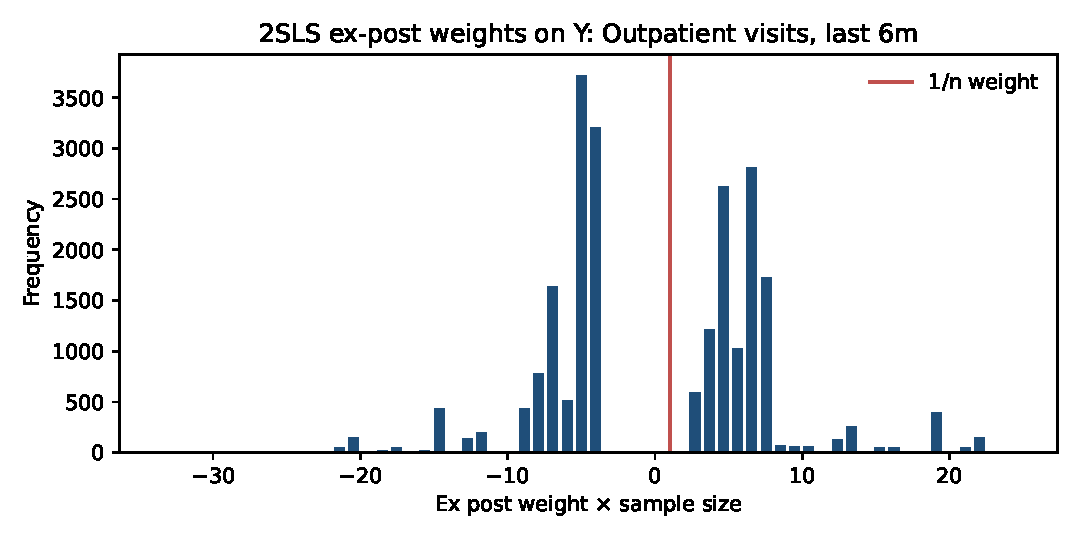
\includegraphics[width=.6\linewidth]{figures/weights_iv_docvisits.pdf}
    \caption{Per-observation 2SLS weights on $Y_{i}$ for outpatient
    visits under the saturated design. Weights are signed: positive on
    treated responders, negative on controls. The balance is what
    enforces the LATE interpretation.}
    \label{fig:iv-weights}
\end{figure}

Figure~\ref{fig:iv-weights} displays weights on the outcome in the
just-identified 2SLS ratio for outpatient visits. Unlike the OLS
effect weights in Figure~\ref{fig:ols-weights}, these are signed
weights on observed outcomes rather than direct weights on individual
treatment effects. Positive weights are attached to observations with
positive residualized lottery status and negative weights to
observations with negative residualized lottery status. The important
diagnostic is therefore not whether every outcome weight is positive,
but whether the residualized instrument is correctly saturated by the
assignment cells. Under the paper's survey-wave-by-household-size
controls, $\E[Z\mid W]$ and the linear projection of $Z$ on $W$ coincide
up to numerical precision; the signed outcome weights then implement
the usual complier-weighted IV contrast rather than introducing an
always-taker term.

% --------------------------------------------------
\subsection{Two-period DiD on the balanced panel}

The balanced 0m--12m survey panel contains $n=16{,}214$ responders to
both the baseline and 12-month surveys, has $T=2$ periods, and a
single, non-staggered treatment date. Under these conditions the
\citet{GB2021} decomposition of the two-way fixed-effect estimator
collapses to a single $2\!\times\!2$ DiD with no ``forbidden''
treated-versus-already-treated comparisons. The TWFE estimand can
therefore be written as a non-negative weighted average of
period-specific average treatment effects on the treated,
\[
    \hat\beta_{\text{TWFE}} \;\xrightarrow{p}\;
    \sum_{t} \frac{C_{t}\cdot \text{ATT}_{t}}{\sum_{t} C_{t}},
    \qquad C_{t}\ge 0,
\]
and is numerically identical (to machine precision) to the two-way
Mundlak transformation of the same regression. I confirm both
properties on the OHIE balanced panel: every individual ex post DiD
weight on $\Delta Y_{i}$ is non-negative, the effective sample size is
$n_{\text{eff}}/n \approx 0.41$, and the TWFE and Mundlak point
estimates agree to fifteen significant digits. The attenuation of the
self-reported-health effect on the balanced panel
($\hat\beta_{\text{ITT}}: 0.039 \to 0.012$; see
\texttt{output/reanalysis\_results.csv}) is therefore due to changing
the analysis sample and adding baseline outcome information, not to
negative TWFE weights.

% ========================================================================
\section{Take-aways}

\begin{enumerate}[leftmargin=*,itemsep=2pt]
    \item OHIE's randomized, stratified encouragement design admits a
        clean heterogeneous-effects decomposition of OLS: ITT
        coefficients are convex combinations of individual effects on
        the treated, omitted-variable bias is exactly zero under
        saturated strata, and ex ante stratum weights concentrate
        around $1/n$ with only modest dispersion.
    \item The 2SLS decomposition of \citet{BBMT2022} shows that the
        $13.5\%$ always-taker share receives no contamination weight in
        the published LATE estimates, because the paper's stratum
        specification saturates the design and forces
        $\E[Z\mid W]=\Lproj[Z\mid W]$. Replacing the stratum dummies
        with a generic linear age-and-sex adjustment reintroduces a
        non-zero contamination weight and shifts $\hat\beta$ by
        roughly $5\%$, matching the BBMT point that 2SLS coincides
        with a LATE only under restrictive
        covariate-balance conditions.
    \item The two-period DiD on the balanced panel exhibits no
        \citet{GB2021} pathology: weights are non-negative and the
        Mundlak/TWFE equivalence holds exactly.
    \item The utilization and financial-protection estimates do not
        change materially in these checks. The self-reported-health
        effect attenuates on the balanced panel, but that check changes
        the sample and conditions on baseline outcomes; it is not
        evidence of negative weighting in the original estimator.
\end{enumerate}

Code, intermediate output, and figures used to produce these results
are in this submission directory; see \texttt{README.md} for a
file-by-file map.

% ========================================================================
\begin{thebibliography}{9}\small

\bibitem[Blandhol et al.(2022)]{BBMT2022}
Blandhol, C., J.\ Bonney, M.\ Mogstad, and A.\ Torgovitsky (2022).
When is TSLS Actually LATE? Working paper.

\bibitem[Finkelstein et al.(2012)]{Finkelstein2012}
Finkelstein, A., S.\ Taubman, B.\ Wright, M.\ Bernstein, J.\ Gruber,
J.\ P.\ Newhouse, H.\ Allen, K.\ Baicker, and the Oregon Health Study
Group (2012). The Oregon Health Insurance Experiment: Evidence from
the First Year. \emph{Quarterly Journal of Economics} 127(3):
1057--1106.

\bibitem[Goodman-Bacon(2021)]{GB2021}
Goodman-Bacon, A.\ (2021). Difference-in-differences with variation
in treatment timing. \emph{Journal of Econometrics} 225(2): 254--277.

\bibitem[Imbens and Angrist(1994)]{IA1994}
Imbens, G.\ W.\ and J.\ D.\ Angrist (1994). Identification and
Estimation of Local Average Treatment Effects. \emph{Econometrica}
62(2): 467--475.
\end{thebibliography}

\end{document}
